\documentclass{beamer}
\usepackage{tcolorbox}
\usepackage{hyperref}
\usepackage{../notation}
\usepackage{pgfplots}
\usepgfplotslibrary{fillbetween}


%\beamerdefaultoverlayspecification{<+->}
% \newcommand{\data}{\mathcal{D}}
% \newcommand\Item[1][]{%
% 	\ifx\relax#1\relax  \item \else \item[#1] \fi
% 	\abovedisplayskip=0pt\abovedisplayshortskip=0pt~\vspace*{-\baselineskip}}

\newcommand*{\Comb}[2]{{}^{#1}C_{#2}}%

\graphicspath{ {imgs/} }

\usetheme{metropolis}           % Use metropolis theme


\title{Ensemble Learning}
\date{\today}
\author{Nipun Batra and teaching staff}
\institute{IIT Gandhinagar}
\begin{document}
	\maketitle
	
	


\begin{frame}{Why combine models?}
\input{test-0.3.tex}
\end{frame}

\begin{frame}{Why combine models?}
% This file was created by tikzplotlib v0.9.0.
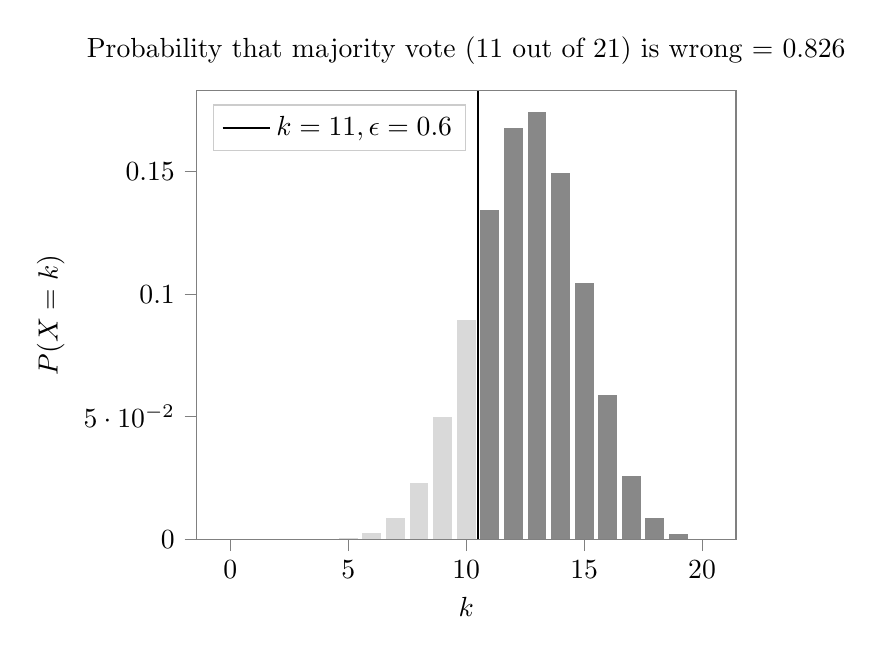
\begin{tikzpicture}

\begin{axis}[
axis line style={white!50.1960784313725!black},
legend cell align={left},
legend style={fill opacity=0.8, draw opacity=1, text opacity=1, at={(0.03,0.97)}, anchor=north west, draw=white!80!black},
tick align=outside,
tick pos=left,
title={Probability that majority vote 
 (11 out of 21) is wrong = 0.826},
x grid style={white!69.0196078431373!black},
xlabel={\(\displaystyle k\)},
xmin=-1.44, xmax=21.44,
xtick style={color=white!50.1960784313725!black},
y grid style={white!69.0196078431373!black},
ylabel={\(\displaystyle P(X=k)\)},
ymin=0, ymax=0.182885197845734,
ytick style={color=white!50.1960784313725!black}
]
\draw[draw=none,fill=white!50.1960784313725!black,fill opacity=0.3] (axis cs:-0.4,0) rectangle (axis cs:0.4,4.39804651110401e-09);
\draw[draw=none,fill=white!50.1960784313725!black,fill opacity=0.3] (axis cs:0.6,0) rectangle (axis cs:1.4,1.38538465099776e-07);
\draw[draw=none,fill=white!50.1960784313725!black,fill opacity=0.3] (axis cs:1.6,0) rectangle (axis cs:2.4,2.07807697649663e-06);
\draw[draw=none,fill=white!50.1960784313725!black,fill opacity=0.3] (axis cs:2.6,0) rectangle (axis cs:3.4,1.97417312767181e-05);
\draw[draw=none,fill=white!50.1960784313725!black,fill opacity=0.3] (axis cs:3.6,0) rectangle (axis cs:4.4,0.000133256686117847);
\draw[draw=none,fill=white!50.1960784313725!black,fill opacity=0.3] (axis cs:4.6,0) rectangle (axis cs:5.4,0.000679609099201017);
\draw[draw=none,fill=white!50.1960784313725!black,fill opacity=0.3] (axis cs:5.6,0) rectangle (axis cs:6.4,0.00271843639680407);
\draw[draw=none,fill=white!50.1960784313725!black,fill opacity=0.3] (axis cs:6.6,0) rectangle (axis cs:7.4,0.00873783127544164);
\draw[draw=none,fill=white!50.1960784313725!black,fill opacity=0.3] (axis cs:7.6,0) rectangle (axis cs:8.4,0.0229368070980344);
\draw[draw=none,fill=white!50.1960784313725!black,fill opacity=0.3] (axis cs:8.6,0) rectangle (axis cs:9.4,0.0496964153790748);
\draw[draw=none,fill=white!50.1960784313725!black,fill opacity=0.3] (axis cs:9.6,0) rectangle (axis cs:10.4,0.0894535476823343);
\draw[draw=none,fill=white!50.1960784313725!black,fill opacity=0.3] (axis cs:10.6,0) rectangle (axis cs:11.4,0.134180321523501);
\draw[draw=none,fill=white!50.1960784313725!black,fill opacity=0.3] (axis cs:11.6,0) rectangle (axis cs:12.4,0.167725401904377);
\draw[draw=none,fill=white!50.1960784313725!black,fill opacity=0.3] (axis cs:12.6,0) rectangle (axis cs:13.4,0.174176378900699);
\draw[draw=none,fill=white!50.1960784313725!black,fill opacity=0.3] (axis cs:13.6,0) rectangle (axis cs:14.4,0.149294039057741);
\draw[draw=none,fill=white!50.1960784313725!black,fill opacity=0.3] (axis cs:14.6,0) rectangle (axis cs:15.4,0.104505827340419);
\draw[draw=none,fill=white!50.1960784313725!black,fill opacity=0.3] (axis cs:15.6,0) rectangle (axis cs:16.4,0.0587845278789856);
\draw[draw=none,fill=white!50.1960784313725!black,fill opacity=0.3] (axis cs:16.6,0) rectangle (axis cs:17.4,0.0259343505348466);
\draw[draw=none,fill=white!50.1960784313725!black,fill opacity=0.3] (axis cs:17.6,0) rectangle (axis cs:18.4,0.00864478351161558);
\draw[draw=none,fill=white!50.1960784313725!black,fill opacity=0.3] (axis cs:18.6,0) rectangle (axis cs:19.4,0.00204744872643526);
\draw[draw=none,fill=white!50.1960784313725!black,fill opacity=0.3] (axis cs:19.6,0) rectangle (axis cs:20.4,0.00030711730896529);
\draw[draw=none,fill=white!50.1960784313725!black,fill opacity=0.9] (axis cs:10.6,0) rectangle (axis cs:11.4,0.134180321523501);
\draw[draw=none,fill=white!50.1960784313725!black,fill opacity=0.9] (axis cs:11.6,0) rectangle (axis cs:12.4,0.167725401904377);
\draw[draw=none,fill=white!50.1960784313725!black,fill opacity=0.9] (axis cs:12.6,0) rectangle (axis cs:13.4,0.174176378900699);
\draw[draw=none,fill=white!50.1960784313725!black,fill opacity=0.9] (axis cs:13.6,0) rectangle (axis cs:14.4,0.149294039057741);
\draw[draw=none,fill=white!50.1960784313725!black,fill opacity=0.9] (axis cs:14.6,0) rectangle (axis cs:15.4,0.104505827340419);
\draw[draw=none,fill=white!50.1960784313725!black,fill opacity=0.9] (axis cs:15.6,0) rectangle (axis cs:16.4,0.0587845278789856);
\draw[draw=none,fill=white!50.1960784313725!black,fill opacity=0.9] (axis cs:16.6,0) rectangle (axis cs:17.4,0.0259343505348466);
\draw[draw=none,fill=white!50.1960784313725!black,fill opacity=0.9] (axis cs:17.6,0) rectangle (axis cs:18.4,0.00864478351161558);
\draw[draw=none,fill=white!50.1960784313725!black,fill opacity=0.9] (axis cs:18.6,0) rectangle (axis cs:19.4,0.00204744872643526);
\draw[draw=none,fill=white!50.1960784313725!black,fill opacity=0.9] (axis cs:19.6,0) rectangle (axis cs:20.4,0.00030711730896529);
\addplot [thick, black]
table {%
10.5 -3.46944695195361e-18
10.5 0.182885197845734
};
\addlegendentry{$k=11, \epsilon=0.6$}
\end{axis}

\end{tikzpicture}

\end{frame}

	\begin{frame}{Ensemble Methods}
	\only<1->{
	Use multiple models for prediction.\\
	Most winning entries of Kaggle competition using ensemble learning.\\
	\vspace{1cm}
	 }
	 \only<2>{
	\textbf{ Example:}\\
	Classifier 1 - Good\\
	Classifier 2 - Good\\
	Classifier 3 - Bad\\
	\vspace{0.5cm}
	Using Majority Voting, we predict Good.\\
	}
	 \only<3>{
	\textbf{ Example:}\\
	Classifier 1 - 20\\
	Classifier 2 - 30\\
	Classifier 3 - 30\\
	\vspace{0.5cm}
	Using Average, we predict $\dfrac{80}{3}$ 
	}
	\end{frame}

	\begin{frame}{Ensemble Methods}
	Error Probability of each model = $\varepsilon$ = 0.3\\
	\vspace{1cm}
	$Pr(\text{ensemble being wrong}) = \Comb{3}{2}(\varepsilon^2)(1-\varepsilon)^{3-2} + \Comb{3}{3}(\varepsilon^3)(1-\varepsilon)^{3-3}$\\
	\vspace{0.5cm}
	\hspace{4.4cm}$ = 0.19 \leq 0.3$ 
	\end{frame}

	\begin{frame}{Ensemble Methods}
	\only<1->{
	Where does ensemble learning not work well?
	}
	\only<2->{
	\begin{itemize}
		\item The base model is bad.
		\item All models give similar or opposite prediction.
	\end{itemize}
	}
	\end{frame}

	\begin{frame}{Bagging}
	\only<1->{
	Also known as $Bootstrap$ $Aggregation$.\\
	}
	\only<2->{
		$Key$ $idea$ : Reduce Variance\\
		\vspace{1cm}
	}
	\only<3->{
		How to learn different classifiers while feeding in the same data?\\
		\vspace{0.5cm}
	}
	\only<4->{
		Think about cross-validation!\\
		\vspace{0.5cm}
	}
	\only<5->{
		We will create multiple datasets from our single dataset using ``$sampling$ $with$ $replacement$''.
	}
	\end{frame}

	\begin{frame}{Bagging}
	\only<1->{
	Consider our dataset has $n$ samples, $D_1, D_2, D_3, \dots, D_n$.\\
	For each model in the ensemble, we create a new dataset of size $n$ by sampling uniformly with replacement.\\
	\vspace{1cm}
	}
	\only<2->{
	Round 1 : $D_1, D_3, D_6, D_1, \dots, D_n$\\
	Round 2 : $D_2, D_4, D_1, D_{80}, \dots, D_3$\\
	\vdots
	}
	\only<3->{
	Repetition of samples is possible.\\
	}
	\only<4->{
	We can train the same classifier/models on each of these different ``Bagging Rounds''.
	}
	\end{frame}

	\begin{frame}{Bagging : Classification Example}
	Consider the dataset below. Points (3,3) and (5,8) are anomalies.\\
	\vspace{0.5cm}
	\centering
	\includegraphics[width = 0.6\textwidth]{dataset}
	\end{frame}


	\begin{frame}{Bagging : Classification Example}
	Decision Boundary for decision tree with depth 6.\\
	\vspace{0.5cm}
	\centering
	\includegraphics[width = 0.6\textwidth]{strong-tree}
	\end{frame}

	\begin{frame}{Bagging : Classification Example}
	Lets use bagging with ensemble of 5 trees.\\
	\vspace{0.5cm}
	\begin{columns}
		\begin{column}{0.3\textwidth}
			\centering
			Round - 1\\
		
			\includegraphics[width = 0.9\textwidth]{dataset-rnd-0}
			
		\end{column}
		\begin{column}{0.3\textwidth}
			\centering
			Round - 2\\
	
			\includegraphics[width = 0.9\textwidth]{dataset-rnd-1}
			
		\end{column}
		\begin{column}{0.3\textwidth}
			\centering
			Round - 3\\
	
			\includegraphics[width = 0.9\textwidth]{dataset-rnd-2}
			
		\end{column}

	\end{columns}
	\vspace{0.5cm}
	\begin{columns}
		\begin{column}{0.3\textwidth}
			\centering
			Round - 4\\
	
			\includegraphics[width = 0.9\textwidth]{dataset-rnd-3}
			
		\end{column}
		\begin{column}{0.3\textwidth}
			\centering
			Round - 5\\
		
			\includegraphics[width = 0.9\textwidth]{dataset-rnd-4}
			
		\end{column}

	\end{columns}
	\end{frame}
	
	
	\begin{frame}{Bagging : Classification Example}
	\vspace{0.3cm}
	\begin{columns}
		\begin{column}{0.3\textwidth}
			\centering
			Round - 1\\
		
			\includegraphics[width = 0.9\textwidth]{decision-boundary-0}
			Tree Depth = 4
			
		\end{column}
		\begin{column}{0.3\textwidth}
			\centering
			Round - 2\\
	
			\includegraphics[width = 0.9\textwidth]{decision-boundary-1}
			Tree Depth = 5
			
		\end{column}
		\begin{column}{0.3\textwidth}
			\centering
			Round - 3\\
	
			\includegraphics[width = 0.9\textwidth]{decision-boundary-2}
			Tree Depth = 5
			
		\end{column}

	\end{columns}
	\vspace{0.5cm}
	\begin{columns}
		\begin{column}{0.3\textwidth}
			\centering
			Round - 4\\
	
			\includegraphics[width = 0.9\textwidth]{decision-boundary-3}
			Tree Depth = 2
			
		\end{column}
		\begin{column}{0.3\textwidth}
			\centering
			Round - 5\\
		
			\includegraphics[width = 0.9\textwidth]{decision-boundary-4}
			Tree Depth = 4
			
		\end{column}

	\end{columns}
	\end{frame}

	\begin{frame}{Bagging : Classification Example}
	Using majority voting to combine all predictions, we get the decision boundary below.\\
	\vspace{0.5cm}
	\centering
	\includegraphics[width = 0.6\textwidth]{decision-boundary-ensemble}
	\end{frame}
	
	\begin{frame}{Bagging}
	\textbf{Summary}
	\begin{itemize}
		\item We take ``strong'' learners and combine them to reduce variance.
		\item All learners are independent of each other.
	\end{itemize}
	\end{frame}
	
	\begin{frame}{Boosting}
	\begin{itemize}
		\item We take ``weak'' learners and combine them to reduce bias.
		\item All learners are incrementally built.
	\end{itemize}
	\end{frame}
	
	\begin{frame}{Boosting : AdaBoost }
	Consider we have a dataset of $N$ samples.\\
	Sample $i$ has weight $w_i$. There are $M$ classifers in ensemble.\\
	\begin{enumerate}
		\item Initialize weights of data samples, $w_i = \dfrac{1}{N}$
		\item For $m = 1\dots M$
		\begin{enumerate}
			\item Learn classifier using current weights $w_i's$
			\item Compute the weighted error, $err_m = \dfrac{\sum\limits_iw_i(incorrect)}{\sum\limits_iw_i}$
			\item Compute $\alpha_m = \dfrac{1}{2}log\left(\dfrac{1 - err_m}{err_m}\right)$
			\item For samples which were predicted correctly, $w_i = w_ie^{-\alpha_m}$
			\item For samples which were predicted incorrectly, $w_i = w_ie^{\alpha_m}$  
			\item Normalize $w_i's$ to sum up to 1.
		\end{enumerate}
	\end{enumerate}
	\end{frame}
	
	\begin{frame}{Boosting: Adaboost}
	Intuitively, after each iteration, importance of wrongly classified samples is increased by increasing their weights and importance of correctly classified 		samples is decreased by decreasing their weights.
	\end{frame}
	
	\begin{frame}{Boosting: Adaboost}
	\textbf{Testing}\\
	Final Prediction = $\alpha_1$(Pred. of Clf. 1) +  $\alpha_2$(Pred. Clf. 2) + $\dots$ +  $\alpha_M$(Pred. Clf $M$)
	\end{frame}
	

	\begin{frame}{Random Forest}
		It is an ensemble of decision trees, where each tree is trained on randomly-selected features.\\
		\vspace{1cm}
		As features are randomly selected, we learn decorrelated trees and helps in reducing variance.\\
	\end{frame}

	\begin{frame}{Random Forest}
	There are 3 parameters while training a random forest ``$number$ $of$ $trees$'', ``$number$ $of$ $features'' (m)$, ``$maximum$ $depth$''.\\
	\vspace{1cm}
	\underline{Training Algorithm}\\
	\begin{itemize}
		\item for $depth$ in $[1, \dots,$ $maximum$ $depth$ $]$
			\begin{itemize}
				\item for $tree$ in $[1, \dots,$ $number$ $of$ $trees$ $]$
				\begin{itemize}
					\item Select ``$m$'' features from total available $M$ features and train a decision tree on selected features
					
				\end{itemize}
			\end{itemize}
	\end{itemize}
	\end{frame}

	\begin{frame}{Code for Examples}
		\centering
		\href{https://colab.research.google.com/drive/1Yix-Hn1zqT6o-wOQkoiBhjKklzhJgekF}{Google Colab}
	\end{frame}


\end{document}